\documentclass[tikz,border=2pt]{standalone}
\usepackage{amsmath}
\usepackage{pgfplots}
\pgfplotsset{compat=1.18}

\begin{document}
% A subsequence keeps some of the terms, in their original order: from a_n = (-1)^n (1 + 1/n)
% the even-indexed terms a_2, a_4, a_6, ... form a subsequence converging to 1.
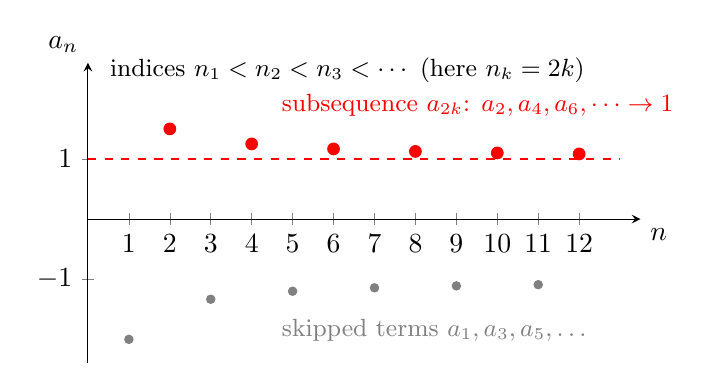
\begin{tikzpicture}
	\begin{axis}[
		axis lines=middle,
		xmin=0, xmax=13.5,
		ymin=-2.4, ymax=2.6,
		xtick={1,...,12}, ytick={-1,1},
		xlabel={$n$}, ylabel={$a_n$},
		xlabel style={below right}, ylabel style={above left},
		clip=false,
		width=8.6cm, height=5.4cm
		]
		\addplot[only marks, mark=*, mark size=1.5pt, gray, samples at={1,3,5,7,9,11}] {(-1)^x*(1+1/x)};
		\addplot[only marks, mark=*, mark size=2.1pt, red, samples at={2,4,6,8,10,12}] {(-1)^x*(1+1/x)};
		\addplot[red, dashed, domain=0:13] {1};
		\node[red, anchor=south west, font=\small] at (axis cs:4.5,1.55) {subsequence $a_{2k}$: $a_2,a_4,a_6,\dots\to 1$};
		\node[gray, anchor=north west, font=\small] at (axis cs:4.5,-1.5) {skipped terms $a_1,a_3,a_5,\dots$};
		\node[anchor=south west, font=\small] at (axis cs:0.3,2.1) {indices $n_1<n_2<n_3<\cdots$ (here $n_k=2k$)};
	\end{axis}
\end{tikzpicture}
\end{document}
